Sensitivity studies presented in Section~\ref{sec:physics-lbnosc-senscalc} test the ability to distinguish
the expected number of \nue appearance and \numu disappearance events given a set of oscillation parameters
from the expectations given an alternate set of parameters. For example, the CP violation and MH sensitivity
studies test the spectral differences induced by shifting \deltacp away from 0.0 and $\pi$ and by changing the
mass hierarchy. These differences are quantified with a test statistic (see Eq.~\ref{eq:dx2_MH}~-~\ref{eq:dx2_CP}) 
which accounts for statistical and systematic uncertainties. 

The effect of systematic uncertainty in the models used to 
predict these spectra is included by allowing the parameters to vary within Gaussian ranges. In the fits,
these systematic nuisance parameters are profiled, i.e., the set of nuisance parameters that produces the
minimum value of the test statistic is chosen.  The central values of the oscillation
parameters and their relative uncertainties are taken from the Nu-Fit~\cite{Gonzalez-Garcia:2014bfa} global
fit to neutrino data; these values are given in Table~\ref{tab:oscpar_nufit}. Uncertainty in non-oscillation
parameters is approximated using
normalization uncertainties on each constituent interaction mode that comprise the signal and background
in each sample. The values for these normalization uncertainties are chosen based on current constraints
on underlying model parameters, the ability of previous experiments to constrain these quantities,
and the expected ability of the DUNE Near Detector (ND) as outlined in Chapter~\ref{ch:detectors-nd-ref}.
Consideration is also given to the sources of uncertainty that go into each of the effective normalization
parameters and how they
may be correlated among the different Far Detector (FD) analysis samples that will be fit in combination.

%In the sensitivities presented in Section ~\ref{sec:physics-lbnosc-senscalc},
%the \nue and \anue signal normalization uncertainties are $5\% \oplus 2\%$, implemented as
%5\% signal normalization uncertainties on the \numu and \anumu samples and
%2\% on the \nue and \anue samples. These four signal normalization uncertainties
%are treated as 100\% uncorrelated so that the 2\% normalization uncertainty on the
%\nue sample represents a residual normalization uncertainty after constraints
%from the near detector, the \numu disappearance samples, and the \anue sample have been applied.
%The normalization uncertainties on background to these samples and the correlation among those
%uncertainties are presented in Table~\ref{tab:bgnormsys}. The result of the correlations
%described in Table~\ref{tab:bgnormsys} is that there are five independent background
%normalization uncertainties: beam \nue, beam \anue, \numu/NC background to appearance mode,
%NC background to disappearance mode, and $\nu_\tau$. 


In the following sections, we present a justification for the chosen values of the signal and background
normalization uncertainties and their respective correlations.
Studies that consider the effect of varying the size of the residual normalization
uncertainties on the \nue and \anue samples are also presented.
Finally we describe the ongoing effort to characterize and evaluate the effect of individual sources
of uncertainty when propagated to oscillation parameter measurements in the DUNE experiment.

\subsection{Far Detector Samples}
\label{sec:syst_just}
Uncertainties in DUNE will be constrained by external data, near detector data, and the combined
fit to the four (\nue appearance, \anue appearance, \numu disappearance, \anumu disappearance) far detector samples.
The \numu disappearance analysis sample is composed of \numu CC interactions with backgrounds from NC
interactions in which a charged pion is misidentified as a muon and $\nu_{\tau}$ CC interactions in which the resulting
tau decays to a muon and two neutrinos.
The unoscillated \numu rate and spectrum are expected to be well-constrained by the near detector.
The uncertainty on the neutral current (NC) background comes primarily from uncertainty in pion production rates
for the coherent, resonance and DIS channels, as well as modeling of pion topological signatures that
determine the likelihood of it being misidentified as a muon.
%The charged pion misidentification rate, and its associated
%uncertainty, is highly correlated with the fraction
%of pions that either exit the detector, are absorbed by nuclei, or expend their kinetic before interacting
%hadronically, and thus have the topological characteristics of a muon.
%These relative rates of these processes will be constrained by the ND.
Uncertainties in the $\nu_{\tau}$ CC background level arise from the uncertainty in the $\nu_{\tau}$/\numu
cross-section ratio, which cannot be directly constrained by ND measurements. Each of these three samples are
assigned a normalization uncertainty. 

The \nue appearance sample is composed of \nue CC interactions resulting from \numu$\rightarrow$\nue oscillation
and background from intrinsic beam \nue interactions, NC and
%high-y$_{bj}$
\numu CC interactions in which a photon from a final-state neutral pion is
misidentified as an electron, and $\nu_{\tau}$ interactions in which the resulting $\tau$
decays to an electron and
two neutrinos. Since the
\numu disappearance signal and the \nue appearance signal are produced by the same flux,
%, flux uncertainty is constrained in the three-flavor fit.
%For example, changing the flux will increase the relative rates of the numu and nue samples the amount,
%while adjusting q23 will cause one sample to rise and the other to fall.
the \nue appearance signal is constrained relative to the \numu
signal. The residual uncorrelated uncertainty on the \nue signal results from the statistical
limitations of the \numu constraint, differences in energy scale and selection efficiency between the samples,
and theoretical uncertainties on the \nue/\numu cross-section ratio.
%These factors all contribute to the \nue signal normalization parameter uncertainty.
The uncertainty on the intrinsic
beam \nue background is dominated by flux uncertainties which are constrained by the near detector and the
observed \numu events.
Predictions for NC and \numu CC background rates are limited by the uncertainties on pion
production rates,
%and the uncertainty assigned to the normalization parameter for the \nue appearance sample combines uncertainties
the $\pi^{0}/\pi^{\pm}$ production ratio, and
differences in selection efficiencies.
%There are correlations between the charged and neutral pion production rates, allowing for
%cancellation of uncertainty in this background between the \nue and \numu samples.
%However, to be conservative the NC+CCnumu backgrounds in the nue are allowed to vary by an additional
%uncorrelated 5% to account for differences in pi0/pi+- production rates, and detection/selection efficiencies.
Again, the $\nu_{\tau}$ background uncertainties are related to cross-section ratio uncertainties
which are treated as 100\% correlated among samples.

The far detector samples for the antineutrino beam mirror those described above for the neutrino beam samples.
Additional constraints are expected to occur in a fit to both neutrino and antineutrino beam samples;
variations in \deltacp induce opposite effects (in both shape and rate) in the \nue and \anue samples,
while most systematic uncertainties have a positively correlated effect.
%Notable correlation considerations between
In the neutrino and antineutrino samples,
NC background to the \numu and \anumu samples is treated as correlated,
as is NC and \numu CC background to the \nue and \anue samples, because the dominant source
of uncertainty is expected to be modeling of pion production.
Signal and beam \nue background normalization is treated as uncorrelated.
The normalization for \nutau CC background is treated as 100\% correlated among all samples.

%% Similar arguments can be made for the antineutrino (RHC) beam samples, and therefore the same effective normalization uncertainties are used. The choice of uncertainties on the effective normalization parameters also reflect the significant cancellations achieved in the 4-sample fit resulting from the addition of 1) relating the nuebar app samples to the numubar dis samples, and 2) from the fact that variations in dcp induce opposite effects (in both shape and rate) in nue and nuebar samples, while most systematics have a positively correlated effect. In these choices it is conservatively assumed that the nu (FHC) flux and the nubar (RHC) flux are not correlated. The only systematic thought to be able to induce an anti-symmetric response between the nue and nuebar samples comes from FSIs. This will require careful constraint from ND analysis, external data, and comparisons of nue to numu, and nuebar to numubar, where the peak of the appearance and the trough of the disappearance samples must be the same. 

Energy scale uncertainties in these samples, which can affect the shape of the reconstructed energy spectra,
result from
inaccurate models of detector response, missing energy in the hadronic systems (primarily from neutron production),
and from final-state interactions (FSI). The dominant source of uncertainty is the hadronic energy scale,
which is the same for both \nue and \numu samples, so relative energy scale uncertainties are limited to
differences in kinematics between \numu and \nue interactions and differences in detector response for
muons and electrons, which will be highly constrained by test beam experiments.
Systematic uncertainties stemming from the FSI model are thought to be able to induce an anti-correlated 
energy scale between the $\nu$ and $\bar\nu$ samples, which has the potential to mimic the effect
of a CP violation signal. However, the effect will be the same in the \nue (\anue) and \numu
(\anumu) samples, allowing the relative \nue to \numu (\anue to \anumu) energy scales to be fixed by comparing
the energies of the appearance peak and the disappearance trough. Additional constraints on the FSI 
model will be required from ND analyses and external data.

\subsection{Anticipating Uncertainties Based on Previous Experience}

Table~\ref{tab:nuesysts} shows the uncertainties in
analyses of \nue appearance rate achieved by MINOS~\cite{Adamson:2013ue}
and T2K~\cite{Abe:2015awa} compared to the goal uncertainties in a similar DUNE analysis.
The goals for normalization uncertainties represent the total expected uncertainty on
an analysis of \nue appearance rate in DUNE; the actual DUNE analysis will be based on
a three-flavor spectral fit to all four far detector samples, so that the portion of these
uncertainties that are correlated among far detector samples is expected to largely
cancel. The portion of these uncertainties that are not correlated among samples and
the effect of energy reconstruction on this analysis must be well understood.
The goals for each source of systematic uncertainty are chosen by determining which
of the existing experiments is more representative of DUNE for that source
of uncertainty and, based on that comparison, setting a reasonable goal for a next-generation
experiment. The goals are based on expected capabilities of the high-resolution
LAr TPC far detector, precise measurements expected from a highly-capable near detector,
and well-understood analysis techniques developed in the existing generation of experiments.
Explanations of the choices in Table~\ref{tab:nuesysts} follow.
%
\begin{cdrtable}[Systematic uncertainty in current experiments]{lcccl}{nuesysts}{
    Systematic uncertainties on the $\nu_e$ appearance
    signal rate prediction in MINOS and T2K and a projection of the
    anticipated uncertainties in DUNE. In each case, the quoted uncertainty is
    the effect on the $\nu_e$-appearance signal rate only. These uncertainties
    are the \emph{total} expected uncertainties on the $\nu_e$-appearance signal
    rate; this includes both those uncertainties that are correlated and those that
    are uncorrelated in the
    three-flavor fit. For reference, the uncertainties assumed in the nominal
    DUNE sensitivity calculations are also provided.}
Source of & MINOS & T2K & DUNE & Comments \\ 
Uncertainty & $\nu_e$ & $\nu_e$ & $\nu_e$ & \\ \toprowrule
Beam Flux & 0.3\% & 3.2\% & 2\% & See ``Flux Uncertainties'' in Section \ref{sec:syst_just_flux}\\
after N/F & & & & \\
extrapolation & & & & \\ \hline
Interaction & 2.7\% & 5.3\% & $\sim 2\%$ & See ``Interaction Model Uncertainties''  \\
Model & & & & in Section \ref{sec:syst_just_sim} \\ \hline
Energy scale  & 3.5\% & included& (2\%) & Included in 5\% $\nu_\mu$ sample normalization\\
($\nu_\mu$) & & above & &  uncertainty in DUNE 3-flavor fit. \\ \hline
Energy  scale & 2.7\% & 2.5\% & 2\% & See ``\nue Energy Scale Uncertainties''\\
($\nu_e$) & & includes & &  in Section\ref{sec:syst_just_fd}\\
 & & all FD & & \\
 & & effects & & \\  \hline
Fiducial & 2.4\% & 1\% & 1\% & Larger detectors = smaller uncertainty. \\
volume & & & & \\  \hline \hline 
Total  & 5.7\% & 6.8\% & 3.6 \% & Residual $\nu_e$ uncertainty in  \\
& & & & full DUNE 3-flavor fit = 1-2\%. \\ \hline \hline
Used in DUNE & & & $5\% \oplus 2\%$ & Residual \nue uncertainty: 2\% \\
Sensitivity & & & & \\
Calculations & & & & \\ 
\end{cdrtable}

\subsubsection{Flux Uncertainties}
\label{sec:syst_just_flux}
DUNE plans to take advantage of spectral analysis,
meaning that absolute and relative flux normalization is required. Since the MINOS \nue appearance analysis
is based on normalization only, in terms of the \nue appearance analysis, DUNE will be more like T2K,
which has achieved 3.2\% normalization uncertainty on their \nue sample from uncertainties in the flux.
Additionally, the inclusive neutrino charged current cross-section measurement from the MINOS
near detector reported in \cite{Adamson:2009ju} has achieved a normalization uncertainty of $\sim$2\% in the
range $3 < E_\nu < 9$ GeV and the near-to-far \numu unoscillated-spectrum extrapolation errors in MINOS
are $<$3\% without any independent constraints on hadron production or muon flux measurements at the near
site. Therefore, as DUNE is planned to have a highly capable near detector, beam line
muon detectors, dedicated hadronization measurements, and improved simulation of beam flux based on
\minerva~\cite{Aliaga:2013uqz} measurements in the NuMI beam, we set a goal uncertainty on \nue signal
normalization from uncertainties in the flux determination of 2\%.
As described in Section \ref{sec:syst_studies_ind}, preliminary simulations of the fine-grained tracker near
detector (ND) suggest this is an appropriate goal, predicting a 2\% uncertainty on the absolute flux and
a 1-2\% uncertainty on the flux shape.

\subsubsection{Interaction Model Uncertainties}
\label{sec:syst_just_sim}
This category of uncertainties arise primarily from uncertainties in modeling neutrino interactions with the target
nuclei in the near and far detectors. These uncertainties include \nue and \numu cross-section uncertainties,
uncertainties from modeling the structure of the target nucleus, and the impact of
hadronization model uncertainties in simulating the break up of the target nucleus in higher-energy inelastic
interactions. DUNE will employ argon nuclear targets in both the near and far detectors, allowing for a larger
cancellation of interaction model uncertainties than in T2K, in which the target nuclei in the near detector are
carbon while those in the far detector are oxygen. Additionally, the angular resolution, vertex resolution,
and particle identification capability of the DUNE near detector are expected to increase its ability to
constrain those cross-section uncertainties which are common between near and far detectors, but for which
the T2K near detector could not provide significant constraint. DUNE's high-resolution near
detector is expected to enable further constraints on hadronization uncertainties, relative to MINOS, by
resolving many of the individual particles produced in the resonance and deep-inelastic scattering interactions
which represent the majority of the DUNE data sample. Finally, significant improvements to neutrino interaction
models are anticipated as a result of the intermediate neutrino program~\cite{Adams:2015ogl},
in which measurements will be made
across a range of different nuclei and the resulting models will be tested on argon in LAr TPCs.
Therefore, we take 2\% as a goal for the effect of
interaction model uncertainties on the DUNE \nue signal normalization. It is important to note that this level of
uncertainty depends upon the ability to isolate neutrino-argon interactions in the near detector to facilitate
cancellation of near-far uncertainties; this is a requirement of the ND design.

Additionally, in considering the effect of the three-flavor analysis on the final uncertainty,
the neutrino beams in DUNE and MINOS have energy
spectra that peak around 2.5-3.0~GeV, compared to 600~MeV in T2K. 
The theoretical uncertainty on the \nue/\numu cross-section ratio is
less than 1\% above neutrino energies of 1.0-1.5 GeV~\cite{Day-McFarland:2012},
a factor of about three smaller than at T2K's median energy,
so the uncertainty on the \nue normalization with respect to the \numu spectrum in DUNE will be
significantly improved compared to T2K. Uncertainty in the $\nu/\bar{\nu}$ cross-section ratio is
somewhat more difficult to quantify given the existing discrepancies between data and currently
implemented models, though this is expected to improve as more complete models are introduced.
As described in Section~\ref{sec:syst_studies_ind}, preliminary studies with a
Fast MC demonstrate the potential for significant cancellation of cross-section uncertainties
in the DUNE three-flavor
analysis, even when uncertainties in the \nue/\numu and $\nu/\bar\nu$ cross-section ratios
are as large as 20\%.

\subsubsection{Uncertainty from \nue Energy Scale}
\label{sec:syst_just_fd}
MINOS and T2K have achieved uncertainty in the \nue signal normalization from \nue energy scale
of 2.7\% and 2.5\% respectively,
where the 2.5\% from T2K actually includes most far detector effects. DUNE's LAr TPC far detector
is expected to outperform both the MINOS sampling calorimeter and the T2K water Cerenkov detector
in reconstruction of \nue interactions. Purity of the quasielastic-like event selection
should be improved relative to T2K by the capability of the LAr TPC to detect hadronic showers
that would be below threshold in SuperK, as described in \cite{Mosel-Lalakulich-Gallmeister:2014}. For non-quasielastic-like
events, the low thresholds and high resolution of the DUNE LAr TPC will significantly improve
calorimetric reconstruction over the MINOS sampling calorimeter.
Significant experience with simulation, reconstruction, and calibration
of neutrino interactions in LAr TPCs is expected from the Intermediate Neutrino Program, particularly
Fermilab's SBN program~\cite{Antonello:2015lea},
which will include three LAr TPCs: SBND~\cite{Admas:2013xka}, $\mu$BooNE~\cite{microboonetdr},
and ICARUS-T600~\cite{Rubbia:2011ft}. An active program of
prototypes and test beam measurements is planned to study the reconstruction of charged and neutral particles
in LAr TPCs; this suite of experiments includes the
DUNE 35-ton prototype (Section~\ref{sec:proto=35t}), LArIAT~\cite{Adamson:2013/02/28tla},
CAPTAIN~\cite{Berns:2013usa}, and
the CERN neutrino platform single (Section~\ref{sec:proto-cern-single}) and dual (Section~\ref{sec:proto-cern-double})
phase prototypes.
Finally, an improved model of neutrino interactions will reduce the impact of imperfect reconstruction
of energy from neutrons and low-momentum protons on the DUNE analysis.
Therefore, we set a goal of using the superior detector performance and the improvements
in understanding of LAr TPC energy response and neutrino interactions
expected in the next 5-10 years to reduce the normalization uncertainty
from the \nue energy scale to 2\%.

In considering the effect of the three-flavor analysis on the final uncertainty, hadronic energy is expected
to contribute more than half of the total energy deposit for many \nue and \numu interactions in the DUNE
far detector. Since the hadronic energy scale does not depend on neutrino flavor, the uncertainties on this
portion of the LAr TPC energy response are expected to largely cancel in the DUNE three-flavor analysis, up
to kinematic differences in the \nue and \numu samples.
The contribution from neutrons will be different between the $\nu$ and $\bar{\nu}$
samples both because of the different
probabilities for neutrinos and antineutrinos to interact with protons and neutrons and because of differing
kinematics. The contribution from neutrons will also be different between the \nue and \numu samples because
these samples peak at different energies due to oscillation effects. For this reason, understanding
of neutron production and detector response to neutrons will be important for constraining uncertainty in
the three-sample fit. Deployment of the CAPTAIN detector in a neutron beam at LANL is planned to address
these issues.


\subsubsection{Total Uncertainties Assigned to the Normalization Parameters}
Based on the preceding considerations, the DUNE signal normalization uncertainty is taken to be
$5\% \oplus 2\%$ in both neutrino and antineutrino mode, where 5\% is the normalization uncertainty
on the FD \numu sample and 2\% is the effective uncorrelated
uncertainty on the FD \nue sample after fits to both near and far detector data and all external constraints.
These signal normalization parameters are treated as 100\% uncorrelated between neutrinos and antineutrinos.
The normalization uncertainties on background to these samples and their respective correlations
are given in Table \ref{tab:bgnormsys}.
These assumptions for the non-oscillation systematic uncertainties 
are used to calculate the sensitivities presented in Section ~\ref{sec:physics-lbnosc-senscalc}.
The goal for the \emph{total} uncertainty on the \nue sample in
DUNE is less than 4\%, so the $5\% \oplus 2\%$ signal normalization uncertainty
used for sensitivity calculations is appropriately conservative.
Additionally, cancellation of the correlated portion of the uncertainty is expected in the four-sample fit, so the
residual uncorrelated normalization uncertainty on the \nue sample is expected to be reduced to the 1-2\% level,
such that the 2\% residual normalization uncertainty used in the sensitivity calculations
is also well-justified. 
Variations on these assumptions are explored in the next subsection.

%
\begin{cdrtable}[Background normalization uncertainties]{lcl}{bgnormsys}{Normalization uncertainties and
correlations for background to the \nue, \anue, \numu, and \anumu data samples.}
      Background & Normalization Uncertainty & Correlations \\ \toprowrule
      \multicolumn{3}{l}{For \nue/\anue appearance:} \\ 
      Beam \nue & 5\% & Uncorrelated in \nue and \anue samples \\
      NC      & 5\%  & Correlated in \nue and \anue samples \\
      \numu CC & 5\% & Correlated to NC \\
      $\nu_\tau$ CC & 20\% & Correlated in \nue and \anue samples \\ \hline
      \multicolumn{3}{l}{For \numu/\anumu disappearance:} \\ 
      NC & 5\% & Uncorrelated to \nue/\anue NC background \\
      $\nu_\tau$ & 20\% & Correlated to \nue/\anue $\nu_\tau$ background \\
  \end{cdrtable}
%

\subsection{Effect of Variation in Uncertainty}
Figure \ref{fig:exp_systs} shows DUNE sensitivity to determination of
neutrino mass hierarchy and discovery of CP violation
as a function of exposure for several levels of signal normalization uncertainty.
As seen in Fig.~\ref{fig:exp_systs}, for early phases of DUNE
with exposures less than 100 kt-MW-years, the experiment
will be statistically limited.
The impact of systematic uncertainty on the CP violation sensitivity for large exposure
is obvious in Fig.~\ref{fig:exp_systs}; the \nue signal normalization uncertainty must
be understood at the level of $5\% \oplus 2\%$ in order to reach 5$\sigma$ sensitivity for
75\% of \deltacp values with exposures less than $\sim$900~kt-MW-years in the case of the
Optimized Design. Specifically, the absolute normalization of the \numu sample must be known to
$\sim$5\% and the normalization of the \nue sample,
relative to the \anue, \numu, and \anumu samples after all constraints from
external, near detector, and far detector data have been applied, must be determined 
at the few percent level. This level of systematic uncertainty sets the capability and
design requirements for all components of the experiment, including the beam design and the
near and far detectors.
%
\begin{cdrfigure}[Variation in sensitivity due to systematics variations]{exp_systs}{
  Expected sensitivity of DUNE  to determination of the neutrino mass
  hierarchy (top) and discovery of CP violation, i.e. $\delta_{CP} \ne$ 0 or $\pi$,
  (bottom) as a function of exposure in kt-MW-years, assuming 
  equal running in neutrino and antineutrino mode, for a range of values for
  the \nue and \anue signal normalization uncertainties from $5\%\oplus3\%$ to
  $5\%\oplus1\%$. The sensitivities quoted
  are the minimum sensitivity for 100\% of \deltacp values in the case of 
  mass hierarchy and 50\% (bottom left) or 75\% (bottom right) of \deltacp values 
  in the case of CP violation. The two bands on each plot represent a range of potential
  beam designs: the blue hashed band is for the CDR Reference Design and the solid green
  band is for the Optimized Design. 
  Sensitivities are for true normal hierarchy; neutrino mass hierarchy
  and $\theta_{23}$ octant are assumed to be unknown.}
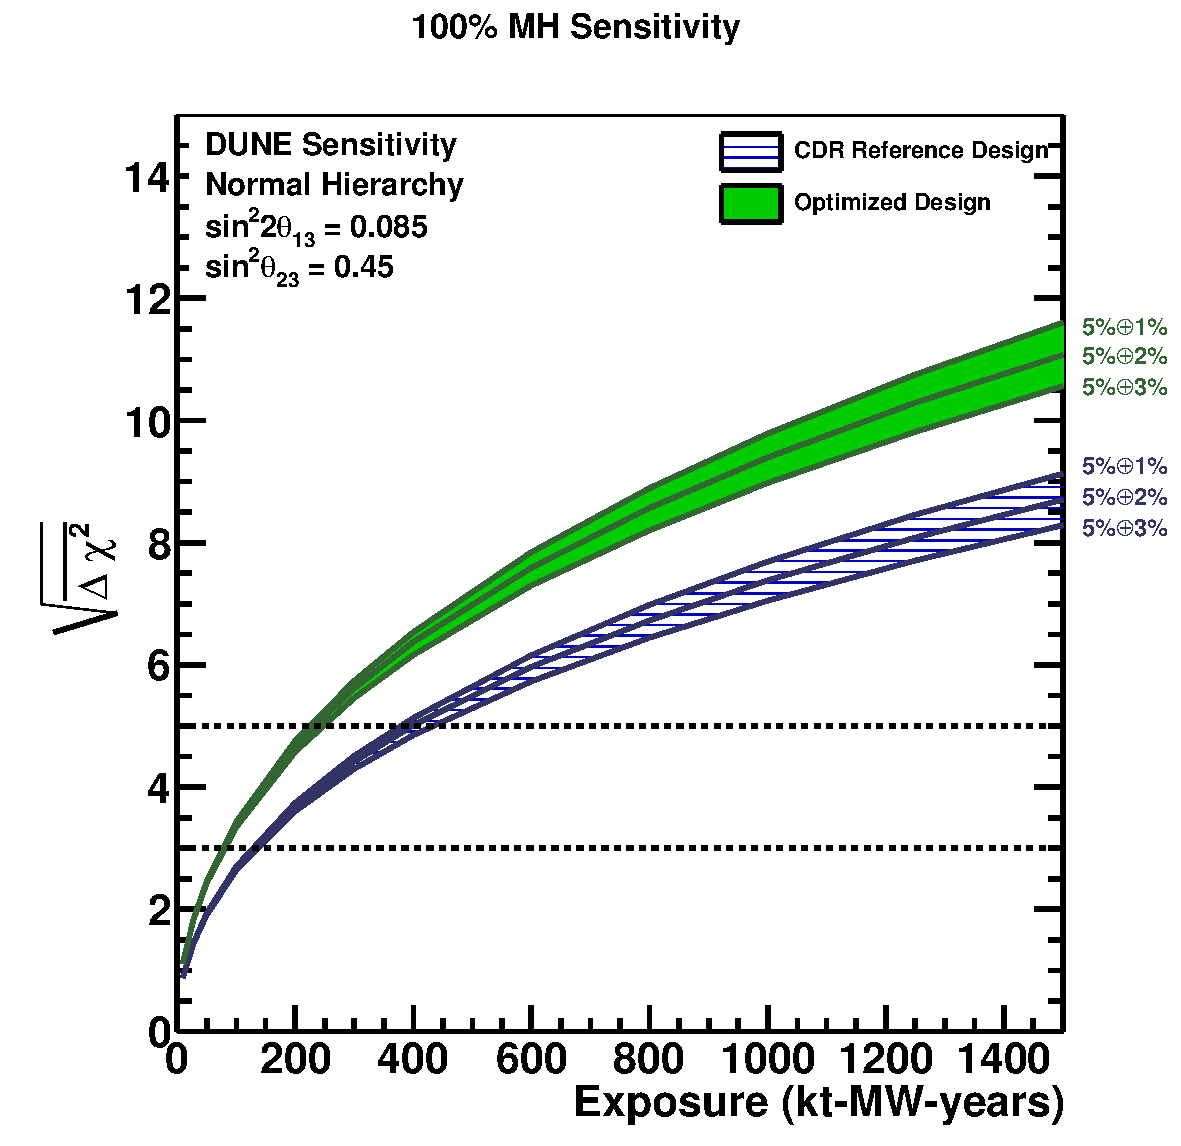
\includegraphics[width=0.45\linewidth]{volume-physics/figures/mh_exp_syst.pdf} \\
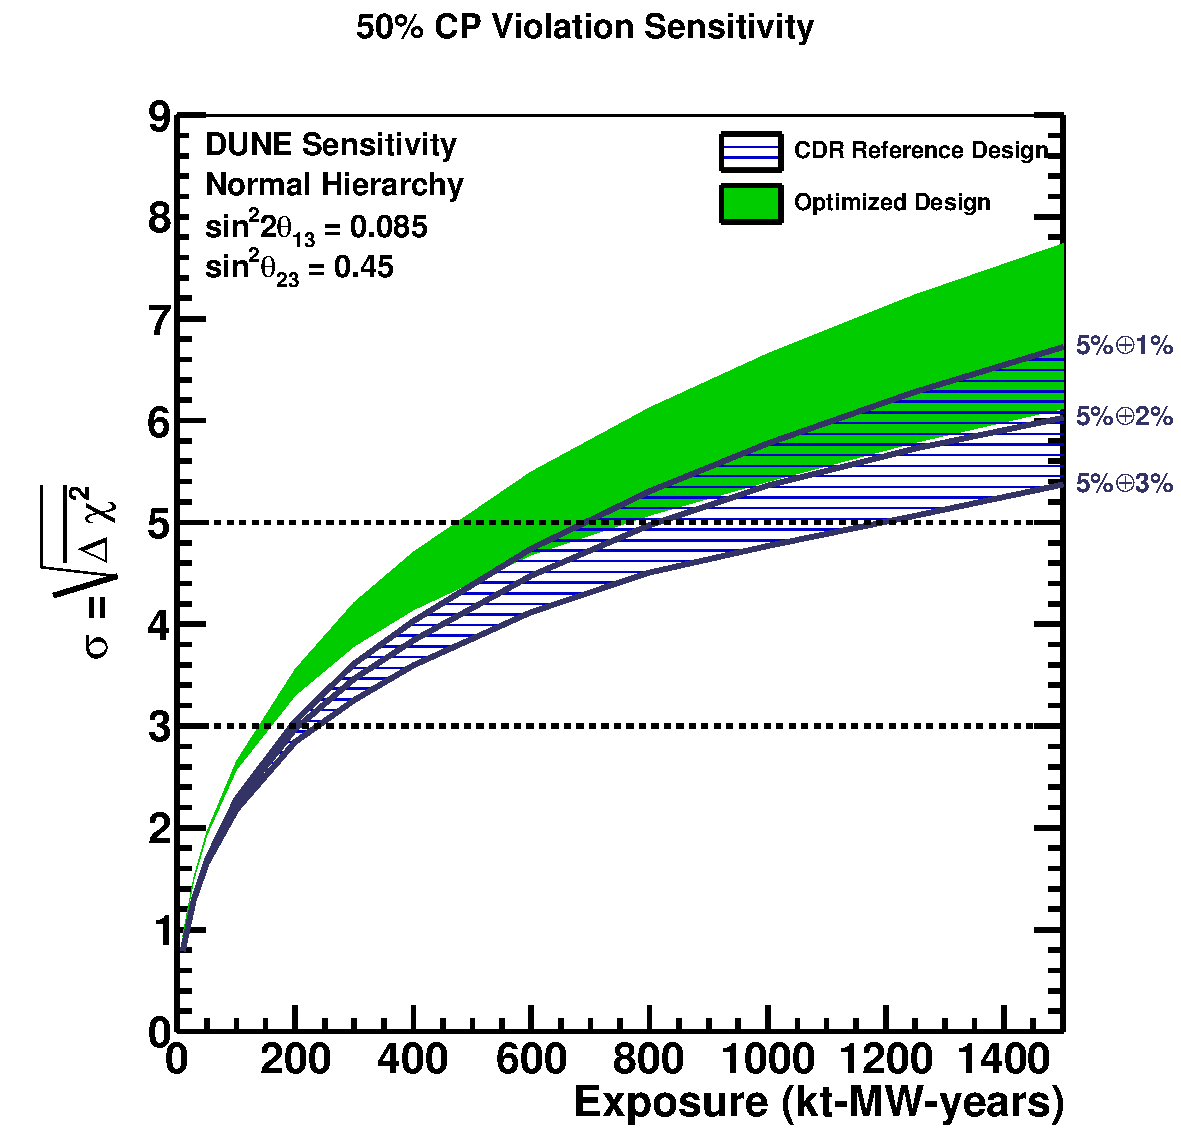
\includegraphics[width=0.45\linewidth]{volume-physics/figures/cpv50_exp_syst.pdf}
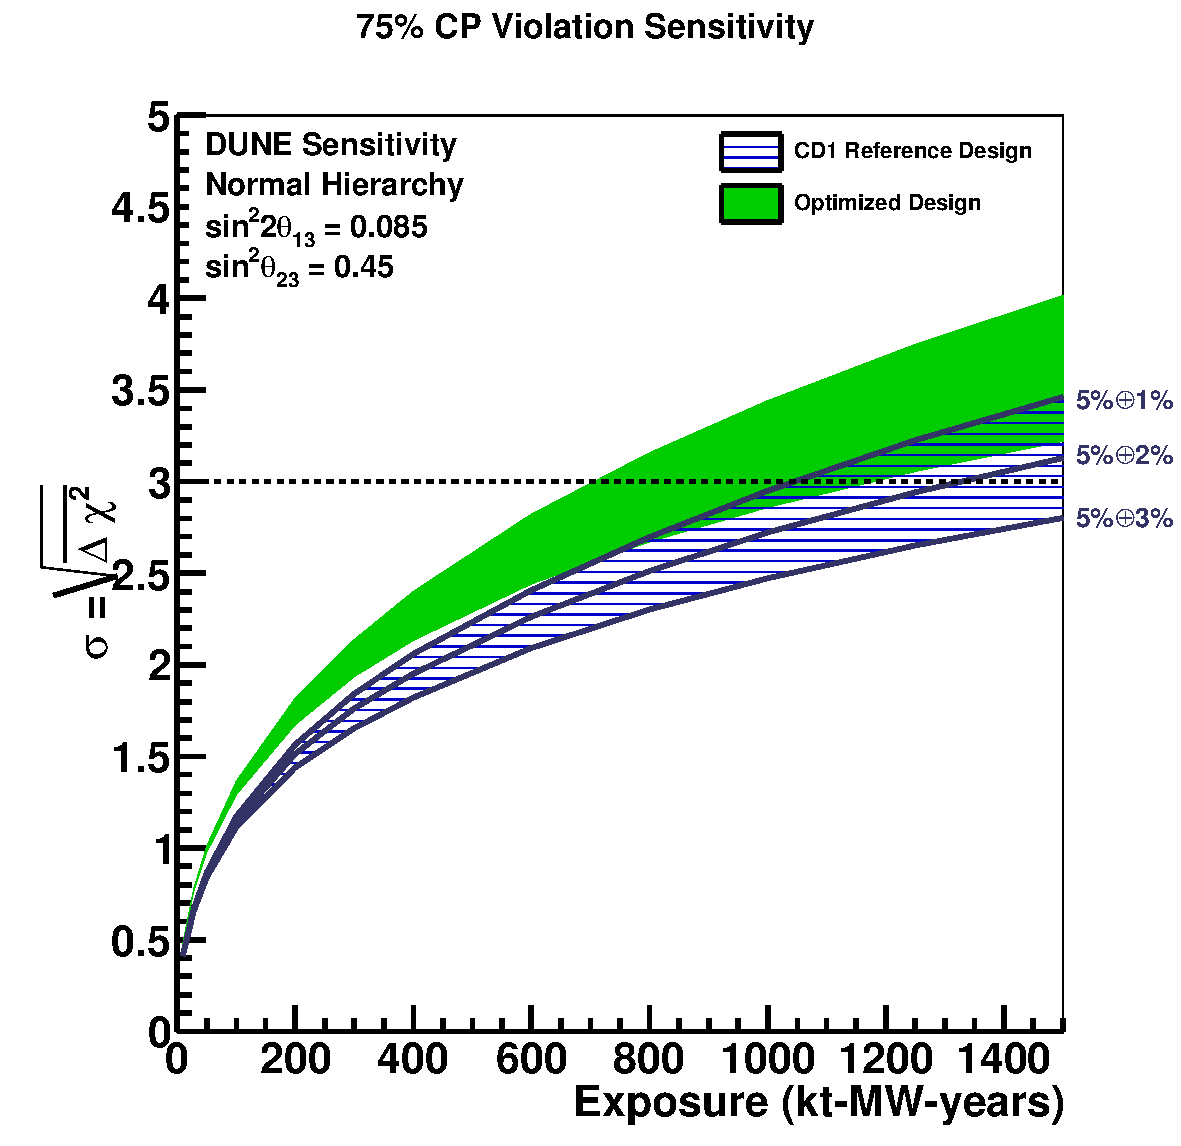
\includegraphics[width=0.45\linewidth]{volume-physics/figures/cpv75_exp_syst.pdf}
\end{cdrfigure}

Signal and
background normalization uncertainties remain
relatively unimportant for the mass hierarchy measurement, even at large exposure, when considering
minimum sensitivity for 100\% of \deltacp values. This is because the minimum sensitivity 
occurs in the near-degenerate region where it is difficult to determine
whether one is observing \deltacp $= + \pi/2 $ in the normal hierarchy
or \deltacp $=-\pi/2$ in the inverted hierarchy. Spectral analysis will
help resolve this near-degeneracy, but is dependent on as-yet
unexplored uncertainties in the spectral shape, which are expected to be dominated
by energy-scale uncertainty. Figure~\ref{fig:escale_syst} shows the
impact on MH and CP violation sensitivity of one possible energy scale variation, in which
energy bins are adjusted by N[E]$\rightarrow$N[(1+a)E], while keeping the total number of
events fixed. This is only one possible type of energy scale uncertainty; more comprehensive
study of energy scale uncertainty is in progress and will be included in
future analyses of experimental sensitivity.
%
\begin{cdrfigure}[Variation in sensitivity due to an energy scale uncertainty]{escale_syst}{
Expected sensitivity of DUNE to determination of the neutrino mass
  hierarchy (left) and discovery of CP violation, i.e. $\delta_{CP} \ne$ 0 or $\pi$,
  (right) as a function of the true value of \deltacp, assuming 
  equal running in neutrino and antineutrino mode, for a range of values assigned to the
  ``a'' parameter in the energy scale variation described in the text. In the MH figure, the case with no
  energy scale systematic provides a significance of at least $\sqrt{\Delta\chi^2}$ = 5 for
  all values of \deltacp. In the CPV figure, the case with no energy scale systematic provides
  a significance of at least 3$\sigma$ for 75\% of \deltacp values.
  (See Figures~\ref{fig:mh_exposure} and \ref{fig:cpv_exposure} for the possible range of exposures
  to achieve this level of significance.)
  Sensitivities are for true normal hierarchy; neutrino mass hierarchy
  and $\theta_{23}$ octant are assumed to be unknown.}
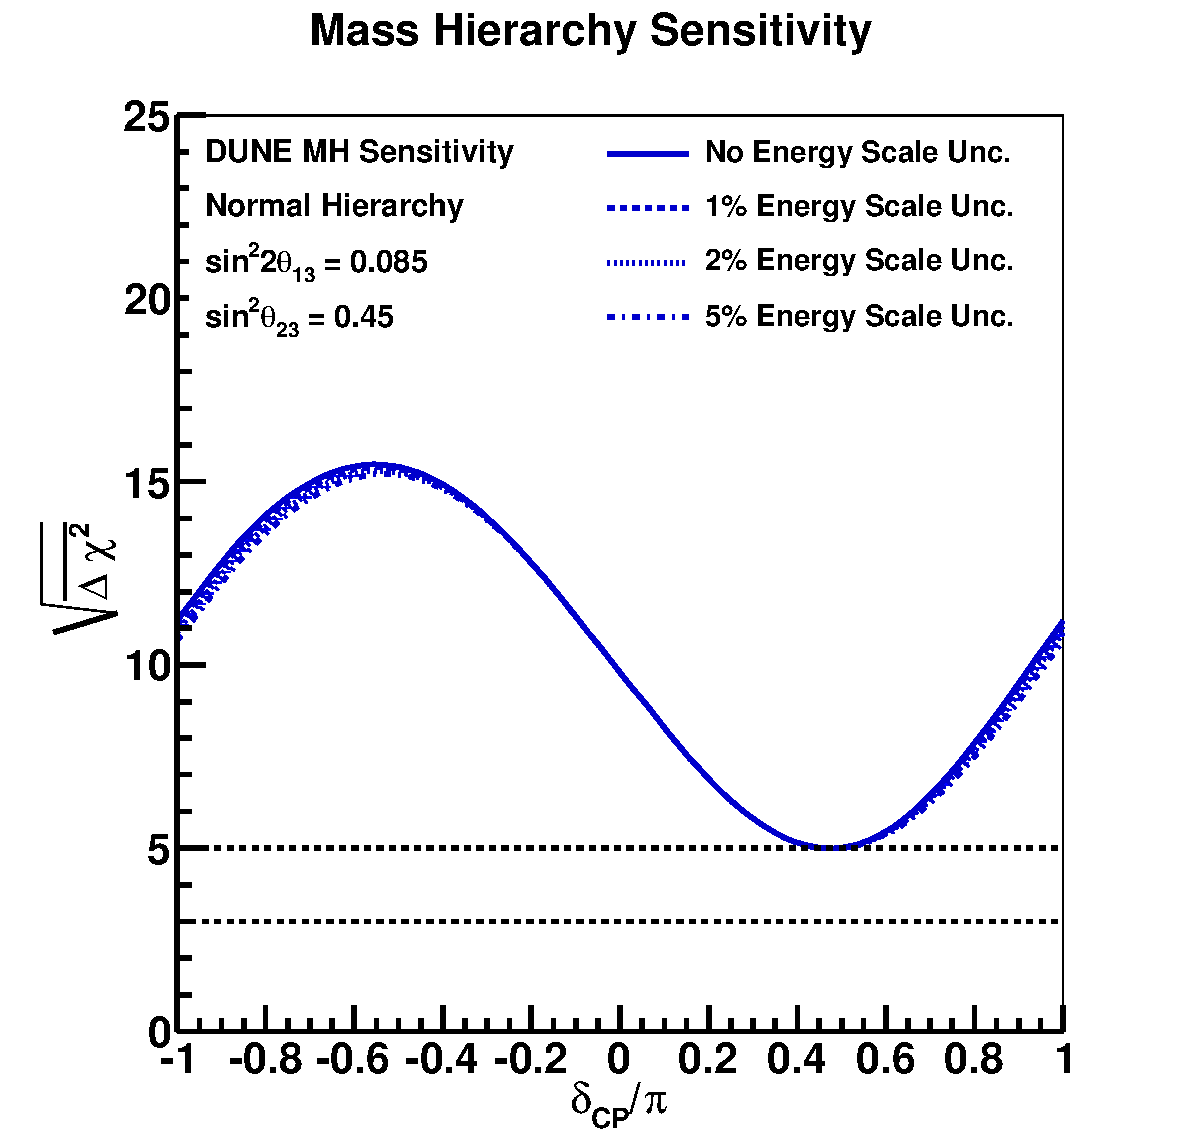
\includegraphics[width=0.44\linewidth]{volume-physics/figures/mh_230ktmwyear_varyesyst.pdf}
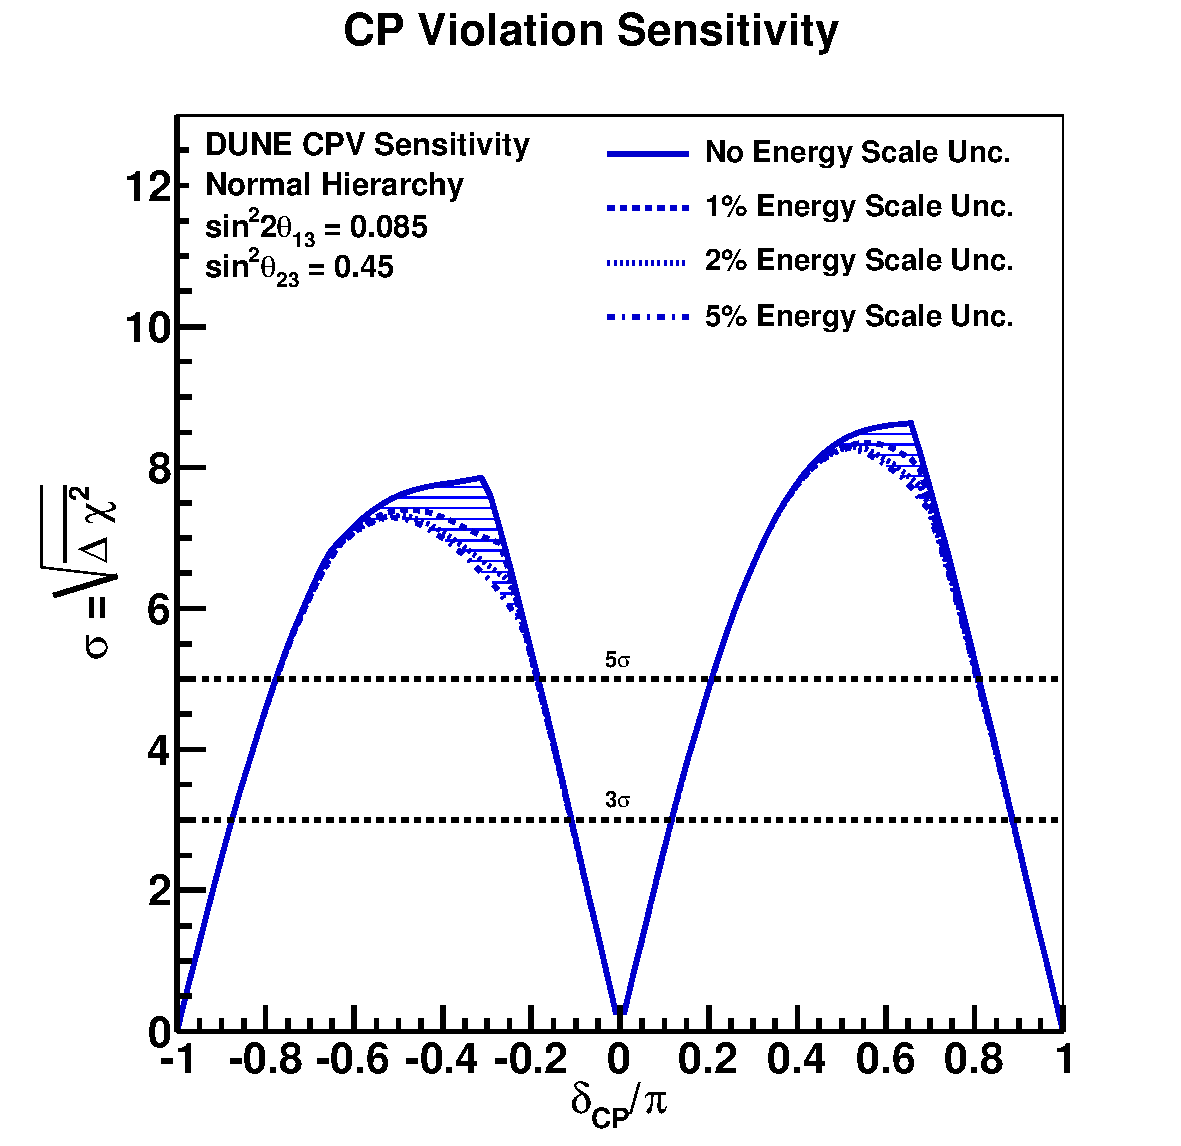
\includegraphics[width=0.44\linewidth]{volume-physics/figures/cpv_890ktmwyear_varyesyst.pdf}
\end{cdrfigure}
%
\subsection{Ongoing and Planned Studies of Systematic Uncertainty}
\label{sec:syst_studies_ind}
Detailed evaluation of systematic uncertainties for DUNE is ongoing. In many cases plans for studies
have been developed but have not yet been executed. In general, each systematic will be studied both by
propagating its uncertainty to oscillation analyses to evaluate the resultant degradation of the sensitivity
and by ensuring the considered variations give proper coverage, i.e., truly encapsulate
the lack of knowledge of the processes/effects in question. Estimates of systematic uncertainty for the 
propagation studies will be varied between the constraints available from current external knowledge
and a range of projections for ND performance. In cases where systematic uncertainty is shown to
degrade the oscillation parameter
measurement sensitivities, the required constraints will become detector performance requirements.
The details of these studies are beyond the scope of this document; however, conclusions from some
initial studies and an overview of each source of systematic uncertainty is laid out in the remainder of
this section.

Initial studies using a Near Detector Fast Monte Carlo with a parameterized detector response
predict 2-3\% statistical uncertainties on the absolute flux using fully 
leptonic neutrino interactions for which high-precision cross-section predictions 
exist. Specifically,
the statistical uncertainty is expected to be 2\% for neutrino-electron
scattering ($E_\nu<5$~GeV) and 3\% for inverse muon decay ($E_\nu>11$~GeV).
Relative normalization using the low-$\nu_0$ method is
expected to constrain the flux shape to 1-2\%; this level of
precision in the \numu flux was achieved by NOMAD\cite{Wu:2007ab,Lyubushkin:2008pe}, enabled by its 0.2\%
uncertainty in the muon energy scale. This flux shape measurement will be made for both \nue and \numu, so,
in combination with measurements from hadron production experiments, can determine the distribution of
the parent mesons which will constrain the near/far flux ratio. Detailed discussion of the planned program
of ND measurements is available in \cite{Mishra:2008nx,Adams:2013qkq}.
Studies using a multi-sample fit  to constrain the flux with simulated DUNE near detector
event samples show significant constraints on all flux
uncertainties; the post-fit uncertainty in most flux bins for this preliminary fit is less
than 5\%, which is the uncorrelated \numu signal normalization
uncertainty assumed by the sensitivity calculations. 

The two main sources of uncertainty in the beam simulation come from variations in the beam optics,
$\mathcal{O}($1\%), and uncertainties in the hadron production models, $\mathcal{O}$(10\%).
Beam optics variations have been studied in detail
%, and while the variations in the flux produced by these uncertainties
%lead to large uncertainties in the FD-only fits,
and are found to be easily constrained by the ND. Software tools that
allow re-weighting of neutrinos based on their parent hadrons have been developed by \minerva; we are working with
them to implement these tools in the DUNE simulation.
In the meantime, \minerva has agreed to provide their flux covariance matrix
that details the flux rate and shape uncertainties prior to ND constraints. We will combine this with DUNE
simulations to project reasonable hadron production uncertainties to ND and FD analyses. Finally,
dedicated hadron production measurements such as those at NA61/SHINE~\cite{NA61:2014fnalbeams}
are expected to reduce these
uncertainties to $\sim$5\%.

Primary interaction uncertainties are specific to each model, and each of the three major
cross-section components (quasi-elastic processes, resonance production, and deep inelastic scattering)
contribute roughly equally to the \nue and \anue
appearance signal. In most cases, uncertainty in modeling primary interactions comes from the
hadronic interaction part of the calculation, which includes form factors in the hadron tensor,
the nuclear initial state, and FSI. 
%The later two sources of uncertainty will be discussed in the context of nuclear models later in this
%section. 

  \emph{Coherent scattering}: Coherent models built upon partially conserved axial current
  theory relate the neutrino scattering 
  cross section to pion-nucleon or pion-nucleus scattering data~\cite{Rein-Sehgal:1983}\cite{Berger-Sehgal:2009}. The choice and characterization
  of that data can have large effects on the calculated cross section. Alternate 'microscopic model' 
  formulations are valid only over limited kinematic ranges and are not adequate to describe this process 
  for DUNE~\cite{Alvarez-Ruso-Geng-Hirenzaki-Vicente-Vacas:2007}\cite{Alvarez-Ruso-Geng-Vicente-Vacas:2007}. 
  Both types of model suffer from limited data constraints over a range of neutrino energy
  and nuclear targets. 
  However, the low hadron thresholds and good angular resolution of the DUNE ND should be able
  to produce world-leading measurements and provide adequate constraints for this interaction channel and 
  its relatively small contribution to the overall cross section. Data from \minerva~\cite{Higuera:2014azj},
  T2K, and
  upcoming LAr TPC experiments will provide constraints for a variety of target nuclei over the
  relevant energy ranges required to constrain this subdominant process.

  \emph{Quasi-elastic processes (QE)}: Models for this type of interaction require that the target nucleon 
  is neither excited nor fragmented because the 4-momentum transfer to the hadronic system ($Q^{2}$) is low.
  For these low-$Q^{2}$ interactions, details of the nuclear initial state are important. However,
  current implementations of nuclear initial state models are inadequate so the uncertainty in the only
  free parameter in the free-nucleon cross-section model, $M_{A}^{QE}$, has been expanded to absorb the
  differences between simulations and $\nu$-nucleus scattering data. Better models of the nuclear
  initial state have been developed
  and are currently being implemented in GENIE and other generators. These new models will be compared with current 
  and future data from \minerva, T2K, and upcoming LAr TPC experiments and the effect of variations in $M_{A}^{QE}$
  on FD spectra will be compared to the effect of introducing the new models.
  Eventually the set of models that best agrees with data will be adopted in the DUNE simulations and
  the uncertainties assigned to these models will reflect the level of agreement with data.

  \emph{Resonance production}:
  There are two important sources of uncertainty in this model. The first is the uncertainty on the free-nucleon
  cross section due to unconstrained form factors and their use as effective parameters to absorb nuclear
  modeling effects.
  The second is the disagreement in outgoing pion kinematics between simulations and data.
  Data from T2K, \minerva~\cite{Eberly:2014mra}\cite{Aliaga:2015wva}, upcoming LAr TPC experiments, and the DUNE ND should provide good constraints for DUNE
  oscillation analyses, but model improvements will be required to help propagate these constraints
  to the FD signal and background predictions. Model improvements are needed for the principal interaction
  model, so-called 'background' interactions where the pion is produced at the interaction vertex
  rather than through an intermediate $\Delta$ (or higher resonance), the interference between the two
  models, and the contributions to single-pion production from low-multiplicity DIS. Improved nuclear models
  are also required to estimate the impact of processes like pion-less delta decay and FSI. New models, which are
  available for some relevant regions of phase space, must be incorporated into generators and compared
  with data~\cite{Hernandez-Nieves-Valverde:2007}.

  \emph{Deep inelastic scattering (DIS)}: The inclusive DIS cross section on iron has been very well constrained by 
  data but individual final states have not. The primary source of uncertainty is in modeling the
  content and kinematics of the hadronic system as a function of its invariant mass. The resulting
  uncertainty on the DIS contribution to signal samples is relatively small, but it is nonetheless important
  to better constrain these models because the DIS contribution to background via pion production is quite large.
  Data from \minerva and upcoming LAr TPC experiments should help to constrain
  the exclusive cross sections, as well as nuclear effects on the inclusive cross section~\cite{Minerva:2014}.
  Current studies are focused on building parameterized re-weighting 
  functions for the hadronization model based on GENIE samples generated with 1$\sigma$ changes to each relevant 
  model parameter.

Nuclear models enter into the simulation of neutrino interactions both through modeling of initial-state interactions,
i.e., interactions between the neutrino and the initial state of the nucleons and virtual particles within the nucleus,
and modeling of final-state interactions (FSI), i.e., interactions of the particles exiting the
primary interaction vertex with the nuclear medium. 

  \emph{Nuclear initial state}: Uncertainties in initial-state interactions due to
  naive modeling of the environment of the nucleus have thus far been taken into account through inflation
  of the uncertainties on the free nucleon or quark interaction
  model. New models~\cite{Alvarez-Ruso-Hayato-Nieves:2014} are being added to generators and will soon be incorporated into the Fast MC
  to study how the impact on sensitivity of these models compares with uncertainties in the current nominal model.
  Data from upcoming LAr TPC neutrino experiments will provide detailed information on nucleon production
  rates and kinematics, which will help to distinguish which of the new models best describes the data.

  \emph{Final-state interactions}: FSI can alter event reconstruction in two distinct ways. The first is a smearing
  of the total energy available to be deposited in the detector. The second is the misidentification of
  event topologies used to classify the neutrino flavor and interaction mode. Uncertainties in selection
  efficiencies and event-sample migrations
  due to intranuclear rescattering can be studied with existing DUNE tools. The predictions and
  uncertainties on GENIE's ``hA'' model~\cite{Dytman:2011zz} of intranuclear interaction
  are being tested against the detailed FSI model in the GiBUU~\cite{Buss:2011mx} event
  generator. Studies of correlations among the free model parameters and and how variations in those
  parameters propagate differently for $\nu$ and $\bar{\nu}$ are also needed. 
  Electron-argon scattering data~\cite{Benhar:2014nca}  and studies of hadron production
  in upcoming LAr TPC experiments are expected to further constrain the effects of FSI in argon nuclei.

A fit to Fast MC simulation of all four far detector samples
(\nue, \anue, \numu, \anumu) significantly
constrains cross-section systematic uncertainty even in the case where many
cross-section parameters are allowed to vary simultaneously within their
GENIE uncertainties. As seen in the example shown in Figure
\ref{fig:MAresqesyst}, 
a fit in which both $M_A^{QE,CC}$ and 
$M_A^{RES,CC}$ are allowed to vary within their GENIE uncertainties 
($\pm$20\%), which could significantly alter the energy distribution of the 
the selected events, results in a dramatic reduction in sensitivity if one 
considers only the $\nu_e$ appearance signal without constraint from the 
$\bar{\nu}_e$ and $\nu_{\mu}$/$\bar{\nu}_{\mu}$ samples.
In contrast, for a four sample fit,
this same parameter variation results in only a small reduction in
sensitivity to CP violation.
This result includes a 10\% uncertainty in the $\nu/\bar{\nu}$
cross-section ratio and a 2.5\% uncertainty in the $\nu_e/\nu_{\mu}$
cross-section ratio; uncertainties in these ratios as large as 20\% have
been considered and did not produce dramatically different results.
More details on this analysis are available in \cite{Bass:2014vta}.
Preliminary studies also demonstrate significant constraint on cross-section systematics
from the near detector.
%
\begin{cdrfigure}[Example of cross-section uncertainty cancellation in FD fit]{MAresqesyst}{
An example CP violation sensitivity calculated using inputs from the 
  FastMC in a fit to all four ($\nu_e$, $\overline\nu_e$, $\nu_{\mu}$, 
  $\overline\nu_{\mu}$) samples (red) and a fit to the $\nu_e$ appearance sample 
  only (blue), for the case of no systematic uncertainty (solid) and the case in
  which both $M_A^{QE,CC}$ and $M_A^{RES,CC}$ are allowed to vary with a
  1$\sigma$ uncertainty of 20\% (dashed). This example was taken from an earlier
  DUNE study, so the absolute sensitivity can not be compared with the DUNE 
  sensitivities presented in this document.}
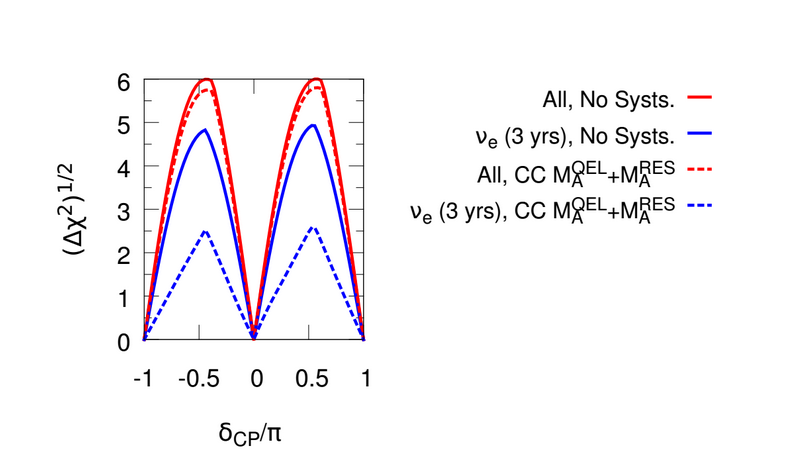
\includegraphics[width=0.8\linewidth]{volume-physics/figures/CPV_MARESQE.png}
\end{cdrfigure}

Uncertainty stemming from detector effects
are somewhat more difficult to address with existing
simulation efforts. Tools to evaluate the effect of uncertainty in single-particle resolutions,
detection and particle-identification efficiencies, and energy scale are in development within
the Fast MC framework. The results of these studies will provide performance requirements
for the DUNE detectors, but more complete understanding of the expected size of these effects
will require comparison between data and a full Monte Carlo.
The status of efforts to develop reconstruction and analysis tools for a full Monte Carlo simulation
of DUNE is described in Section~\ref{sec:detectors-sc-physics-software}. At the same time,
a number of test-beam and prototype experiments, including the DUNE 35-t prototype,
LARIAT, CAPTAIN, and the CERN neutrino platform experiments, are being designed and built to reduce these
uncertainties with experimental data. The status of some of these efforts is described in
Chapter~\ref{ch:detectors-proto}.

These ongoing studies to improve models of neutrino interactions in LAr TPC detectors and
to evaluate the remaining uncertainties, by comparisons to data and alternate models, 
are a high priority of the whole neutrino community as well as the DUNE collaboration.
It is reasonable to expect that model improvements and new data will provide DUNE with improved inputs
and reduced uncertainties compared to current knowledge. Following the plan described in the preceding
paragraphs, DUNE collaborators will actively participate in the global effort to improve understanding
of neutrino interactions, will propagate what is learned
in the intermediate neutrino program to DUNE analyses, and will
evaluate the effect of remaining uncertainties on the DUNE analyses.









